
We will now present the results of narrow set of experiments aimed to observe both user confort when exposed to different visualization conditions offered by our application (chosen among all the possible setups provided) and to measure performance where the vision pipeline is active.

As a common setting, the 3D rendering engine has been forced to run at 60 fps while each camera runs at its best with 30 fps.  Performance results will be classified by computational hardware used, application setting and camera image resolution.

A consideration must be done for camera resolution. With cameras in stock configuration, the highest 16:9 resolution used in the experiments is 1024x576 (on the 1920x1080 available): the reason is that, since image will not cover the entire HMD FOV with stock wide-angle lenses, it is no use to use the whole sensor surface. Resolution was then further reduced whenever the subject could not perceive any loss in quality (thus improving performance at zero cost) or whenever we needed to experiment with performance to provide more complete results or a reasonable frame rate with hardware in use.\\
The high resolution of the sensor however still comes in handy when dealing with fish-eye lenses: to achieve the highest FOV possible, it is convenient to adjust the lens so that the entire fish-eye circle is restricted into the 16:9 area of the sensor used for video streaming, which in turn explains the need of higher resolution (image will need to be scaled to cover the entire HMD screen).

First tests were conducted on an Asus U500VZ, Intel i7 3632QM (four cores) CPU clocked at 2.8 Ghz and 8GB RAM, Nvidia GT650M with 2GB RAM.
Latest tests with CUDA and demo were conducted on "Aragorn" (from CVAP), Intel i7 3930K (six cores) CPU clocked at 3.20GHz and 32GB RAM, Nvidia Tesla K40c with 12GB RAM.

\section{Live stereo augmented reality demo}
In this experiment we tested the behaviour of the application in wide-angle toed-in configuration, streaming live images from the cameras into the HMD, and presenting them to the user. In this demo we feature a version of the application meant to study the impact of AR video see-through (in our specific setup) on multiple subjects, volunteering out of curiosity or sincere interest in the project, and to test the model and architecture capabilities. Features provided were:
\begin{itemize}
\item camera pose stabilization: can be turned on and off to test its impact on the subject;
\item skybox: meant to test discrepancy between head movements and image delay plus enhancing comfort, also can be turned on and off;
\item camera image undistortion and marker detection for augmented reality: demonstration of discrepancy reduction in depth perception between virtual and real objects and highlighted its limits;
\item "toon shading" effect: showed off CUDA filtering capabilities and impact on performance and user perception in Non-PhotoRealistic rendering conditions.
\end{itemize}

To 20 subjects has been asked to walk around in a room with HMD on and to provide feedback, test demo configurations and experience 3D perception when watching the marker static or manipulating it. To better understand how video see-through and immersive AR experience can be improved, the application has been structured in steps (figure \ref{fig:demo_steps}). The first step has four configurations, starting from the bare minimum image visualization: subjects can freely switch between each other on personal preference and provide personal opinion and express discomfort, if any. Users were specifically asked to rotate their head around to identify the difference between stabilized and non-stabilized mode and then move on with activating the skybox.

\begin{figure}
\centering
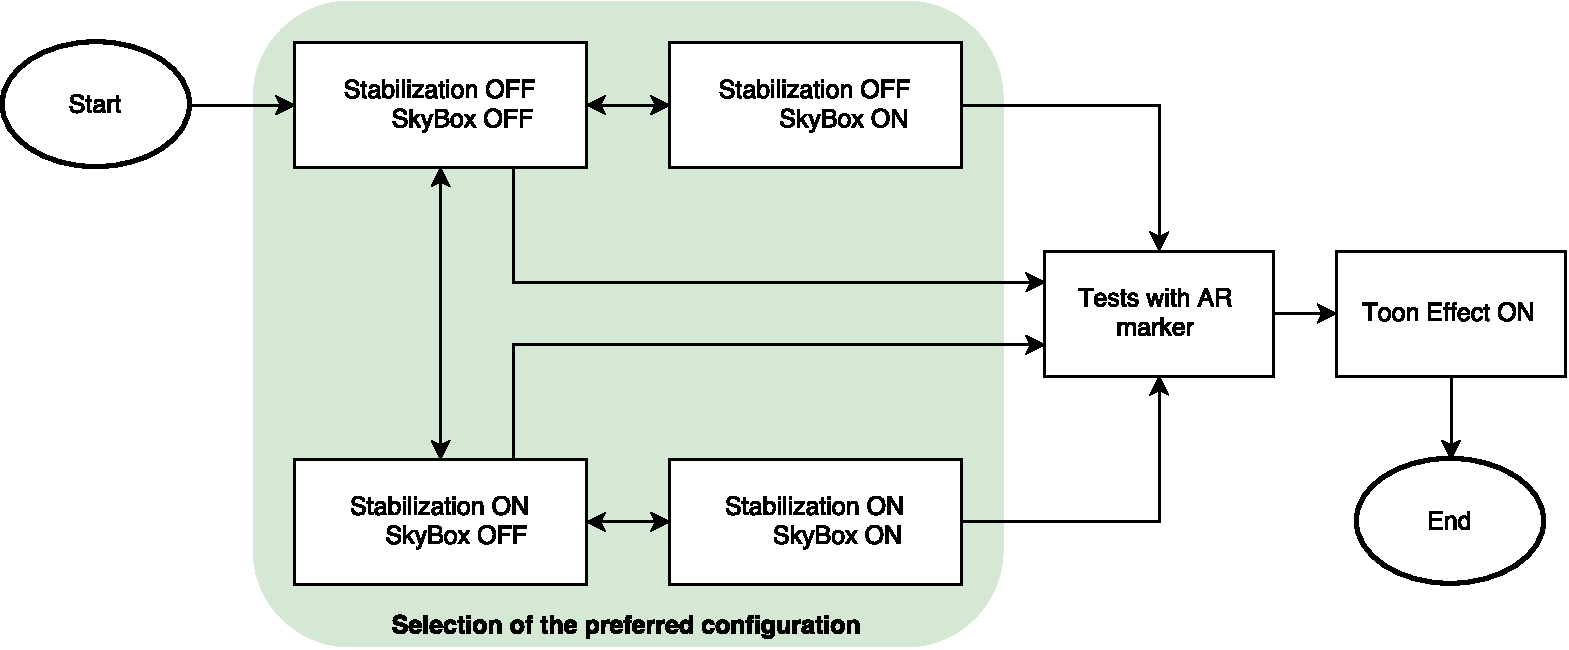
\includegraphics[width=\linewidth]{schemas/demosteps}
\caption{Graphical representation of steps of the experiment. Arrows indicate which path and in which direction can be taken from a state to another.}
\label{fig:demo_steps}
\end{figure}

Once most confortable setup is chosen, the marker is placed in view and is given to the user the chance to manipulate it. As a result, previously mentioned geometrical problems revealed themselves in form of AR virtual object and AR marker mismatches. This offered a good excuse to play around with base application settings, meant exacly to overcome such limitations. With the help of users' feedback we could confirm that for every distance between actor and marker existed a set of settings that could solve virtual/real discrepancy for that distance. In particular, the setting that allowed to adjust perceived zero-parallax distance (by toeing in the image planes) was effective. With an on-the-fly hack was able to mitigate the problem by dynamically adjusting the plane toe-in angle in respect to detected distance of the marker from camera used for AR by linear approximation. Keystoning was not really noticed by anyone until problem was pointed out by us.

As final bonus, the effect pipeline was activated (with toon shading embedded in the demo). Final resolution of “cartoonized” camera image was chosen so that it was the closest to the original and achieved lower framerate. This way, subjects could both experience NPR environment and be exposed to the impact on performance with the chosen configuration. As algorithm stabilization still worked well, since it merely reproduces original image pose and time capture estimation did not change, but all subject noticed image plane additional jerking and found it discomforting. However, we do not suggest to implement any kind of interpolation: this would make plane move more smoothly, but the image will still remain static and the mismatch we worked hard to remove will again be there. Instead, cameras with a higher FOV should be used in order to hide completely image borders.

We have classified (in table \ref{demo_subject_classes}) the users which span from highly sensitive (which means they have preemptively declared they had past experiences with HMDs and VR or stereo content, not satisfactory) to people entirely new to the subject.

\begin{table}[]
\centering
\begin{tabular}{llll}
Class 1                                                                          & Class 2                                                                          & Class 3                                                                           & Class 4                                                                          \\
\multicolumn{1}{c}{\cellcolor[HTML]{FFBCA4}{\color[HTML]{E10000} \textbf{3/20}}} & \multicolumn{1}{c}{\cellcolor[HTML]{FFD453}{\color[HTML]{F56B00} \textbf{4/20}}} & \multicolumn{1}{c}{\cellcolor[HTML]{9AFF99}{\color[HTML]{009901} \textbf{10/20}}} & \multicolumn{1}{c}{\cellcolor[HTML]{ECF4FF}{\color[HTML]{6434FC} \textbf{3/20}}}
\end{tabular}
\caption{Subjects classified on previous experience with Oculus Rift. Class 1: have tried and experience sickness; Class 2: have tried and could withstand; Class 3: have never tried, but report to be gamers; Class 4: have never tried and have no gaming habits.}
\label{demo_subject_classes}
\end{table}

The premise is the experiment could be considered a success whenever the majority of subjects voted for the expected preferred configuration. Keep in mind that, for technical limitations, the setup presented was using toed-in pin-hole camera model and wide-angle lenses, so not the best according to what discussed so far. The results are however still relevant considering that toe-in is still a common configuration, for stereo computer vision (reasonably) and stereo imaging reproduction (erroneously). Since a focus for future stereo computer vision algorithms development is given, we welcome the level of challenge of optical issues involved.

\begin{table}[]
\centering
\caption{Perceptual results from Step 1 of the experiment. Order expresses class and number how many subjects for each class selected that configuration.}
\label{perceptual_results}
\begin{tabular}{c|c|c}
           & Stabilization OFF                                              & Stabilization ON                                               \\ \hline
Skybox OFF & \begin{tabular}[c]{@{}c@{}}0/3\\ 1/4\\ 1/10\\ 0/3\end{tabular} & \begin{tabular}[c]{@{}c@{}}0/3\\ 0/4\\ 1/10\\ 1/3\end{tabular} \\ \hline
Skybox ON  & \begin{tabular}[c]{@{}c@{}}0/3\\ 0/4\\ 0/10\\ 0/3\end{tabular} & \begin{tabular}[c]{@{}c@{}}3/3\\ 3/4\\ 8/10\\ 2/3\end{tabular}
\end{tabular}
\end{table}

A table of perceptual results for first step is given in figure \ref{perceptual_results} in sample and class. Results demontrate how only a majority of the sample completely agree that the proposed improvements helped in feeling the right response between head movement and image, while the minority quite naturally disagreed, expressing discomfort when exposed to strategies implemented so far addressing them as "distracting elements". Few exceptions in the end did not feel the difference at all, until asked to force the hand on purpose. AR pose estimation is among the understandable complaints since it is prone to detection errors that depend on multiple factors out of our reach, like illumination, camera image quality or the effective mismatch between a real rotation of the cameras and a virtual rotation of the head. As for the other two aspects, further investigation indicates that discrepancy, of any entity, disrupts immersion: image plane is indeed limited and users could appreciate this aspect only after a rescaled image was presented to the eyes. At that point, we explained how higher FOV cameras or even better fish-eye lenses could cover the whole view, thus hiding edges and making skybox apparently not necessary.

Whether or not the stabilization step was preferred, we took care in explaining how such aspect could be appreciated: switching between stabilized skyboxed and non-skyboxed, most subjects (15/22) have been able to realize how discrepancy between image (laggy) and background (reactive) is tackled when focusing on the image content and not the frame bounaries. The same effect can also be noted on stabilized non-skyboxed, by focusing on a real object then turning head suddenly and see the reaction, and with AR virtual object when moving head fast, being able to "follow" better the underlaying marker.

Major issue encountered in experiments is discrepancy between marker pose and perceived virtual object position in space. We feel confident that this is a geometrical problem that can be formulated and can exploit the image plane meshes approach to correct undesired effect under current condition, even though it will inevitably fail with more markers to be detected at a time (which is the one in view to be used as stereo matching reference?). This gave us further motivation to our design choice, where cameras are toed-in for optimal stereo computer vision and the optimal working distance can be tweaked manually at runtime (instead of needing to toe-in cameras at a different angle).

Performance was less criticized. 3/22 subjects pointed out there were lag problems (excluding people that referred to camera stabilizaion as the latency issue itself) but not at the point application was unusable. Different question is the the toon filter applied: there was a noticeable drop in camera FPS (not influencing Ogre's FPS) which forced us to reduce its size for the image effects pipeline, while marker detection still uses the same. The choice of 640x360 satisfied everyone and did not look as a loss at all given the kind of elaboration to be done with it.

\section{CUDA pipeline performance with NPR filter}
In the demo from previous paragraph has been activated the image effect pipeline, which uses the camera image and CUDA support to apply a Non-Photorealistic-Reality (NPR) filter. Gooch shading was also used to apply a "toon" effect to the rest of the virtual environment.

In this case, any experimentation focused more on performance measurement than user experience, since deeper research and control over virtual environment rendering output is needed to achieve reliable results in terms of psychological perception. We asked anyway a less formal opinion on subjects under test on whether they could still distinguish real objects (from camera image) from the virtual object (from AR pipeline): as far as the virtual object overlayed on the image and the user was almost static, it seemed really hard to tell the difference under our conditions. Tests were performed with both OpenCV undistortion on and off. Undistortion, toghether with image effects and enhancement, should be implemented in CUDA. With our setup, arUco was successful in detecting the marker properly even without undistortion. In any case, the undistortion implemented is an optimized version \cite{link_optimized_undistort_opencv} In table \ref{performance_image} we report the times of execution for each processing stage and the achieved frame rates for two different cases. Note that at all cases, 3D rendering frame rate kept on stable 60 fps.

\begin{table}[]
\centering
\begin{tabular}{c|c|c|c|c}
                                                                    & \multicolumn{1}{l|}{1920x1080} & \multicolumn{1}{l|}{1024x576} & \multicolumn{1}{l|}{768x432} & \multicolumn{1}{l}{512x288} \\ \hline
\begin{tabular}[c]{@{}c@{}}cv::undistort\\ (optimized)\end{tabular} & 18ms                           & 11ms                          & 7ms                          & 5ms                         \\ \hline
aruco::detect                                                       & 28ms                           & 15-16ms                       & 11ms                         & 8ms                         \\ \hline
CUDA pipeline                                                       & 42ms                           & 24ms                          & 20ms                         & 16ms                        \\ \hline
FPS no/fx                                                           & 26-28fps                       & 30fps                         & 30fps                        & 30fps                       \\ \hline
FPS with/fx                                                         & 9-10fps                        & 17fps                         & 24fps                        & 28fps                      
\end{tabular}
\caption{All measurements are made on "Aragorn" and have to be intended as average and per each camera thread. The frame rate instead measure keeps count of both cameras running. The processor on which the test run supported multi-threading and TBB was used by OpenCV.}
\label{performance_image}
\end{table}

To run our demo for perceptual tests, we fixed cameras running at 1024x576 (also because without high FOV lenses, using more is a waste) and CUDA pipeline to work with a reduced version of 512x288 to keep performance reasonable (with the "toon" effect on, any reduction of resolution of source image is less noticeable anyways).


\section{Offline stereo fish-eye demo}
Since in our experiments we did not have reasonable control over lens replacement and positioning on stock cameras, we proposed an alternative able to test the capabilities of our fish-eye mesh undistortion algorithm implemented in a GLSL fragment shader. The demo application (if specified) can run in "Fish-eye" mode, bypassing the standard "Pin-hole" setting. The application loads by default a fish-eye stereo pair, to experiment with shader calibration. Manual operations possible are aspect-ratio, translation scale of the texture for each eye (details are described in the documentation), which dynamically adjust the relevant parameters mentioned in Chapter 3.
No experiments were issued in this modality, since stereo calibration, when performed manually, could lead to very personal results. Moreover, without marker detection or AR in general, it is impossible to experiment virtual-real discrepancies in this state, even though the same adjustments are allowed.



